%
%   This program is free software: you can redistribute it and/or modify
%   it under the terms of the GNU General Public License as published by
%   the Free Software Foundation, either version 3 of the License, or
%   (at your option) any later version.
%
%   This program is distributed in the hope that it will be useful,
%   but WITHOUT ANY WARRANTY; without even the implied warranty of
%   MERCHANTABILITY or FITNESS FOR A PARTICULAR PURPOSE.  See the
%   GNU General Public License for more details.
%
%   You should have received a copy of the GNU General Public License
%   along with this program.  If not, see <http://www.gnu.org/licenses/>.
%

% Version: $Revision$

The Weka GUI Chooser (class \texttt{weka.gui.GUIChooser}) provides a
starting point for launching Weka's main GUI applications and
supporting tools. If one prefers a MDI (``multiple document
interface'') appearance, then this is provided by an alternative
launcher called ``Main'' (class \texttt{weka.gui.Main}).

%%The new menu-driven GUI in WEKA (class \texttt{weka.gui.Main}) succeeds the old GUI Chooser (class \texttt{weka.gui.GUIChooser}). Its MDI (``multiple document interface'') appearance makes it easier to keep track of all the open windows. If one prefers an SDI (``single document interface'') driven layout, one can invoke this with option \texttt{-gui sdi} on the commandline.

The GUI Chooser consists of four buttons---one for each of the four
major Weka applications---and four menus. 

\begin{center}
	\includegraphics[angle=270,width=5cm]{images/launching/GUIChooser.eps}
\end{center}

The buttons can be used to start the following applications:

		\begin{itemize}
			\item \textbf{Explorer} An environment for exploring data with
WEKA (the rest of this documentation deals with this application in more detail).
			\item \textbf{Experimenter} An environment for performing experiments and conducting statistical tests
between learning schemes.
			\item \textbf{KnowledgeFlow} This environment supports essentially
the same functions as the Explorer but with a drag-and-drop
interface. One advantage is that it supports incremental learning.
			\item \textbf{SimpleCLI} Provides a simple command-line interface
that allows direct execution of WEKA commands for operating systems
that do not provide their own command line interface.
		\end{itemize}




The menu consists of four sections:

\begin{enumerate}
	\item \textbf{Program} \\
	        \includegraphics[angle=270,width=2cm]{images/launching/guic_program.eps}
		\begin{itemize}
			\item \textbf{LogWindow} Opens a log window that captures all that is printed to \textit{stdout} or \textit{stderr}. Useful for environments like MS Windows, where WEKA is normally not started from a terminal.
			\item \textbf{Exit} Closes WEKA.
		\end{itemize}
				
	\item \textbf{Tools} Other useful applications. \\
                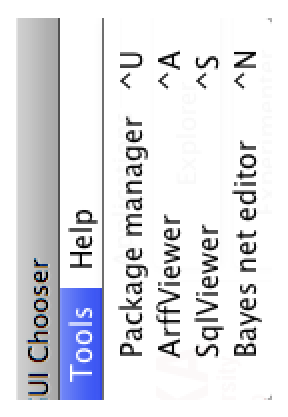
\includegraphics[angle=270,width=2cm]{images/launching/guic_tools.eps}
		\begin{itemize}
                        \item \textbf{Package manager} A graphical interface to Weka's package management system.
			\item \textbf{ArffViewer} An MDI application for viewing ARFF files in spreadsheet format.
			\item \textbf{SqlViewer} Represents an SQL worksheet, for querying databases via JDBC.
                        \item \textbf{Bayes net editor} An application for editing, visualizing and learning Bayes nets.
		\end{itemize}
		
	\item \textbf{Visualization} Ways of visualizing data with WEKA. \\
		\includegraphics[angle=270,width=2cm]{images/launching/guic_visualization.eps}
		\begin{itemize}
			\item \textbf{Plot} For plotting a 2D plot of a dataset.
			\item \textbf{ROC} Displays a previously saved ROC curve.
			\item \textbf{TreeVisualizer} For displaying directed graphs, e.g., a decision tree.
			\item \textbf{GraphVisualizer} Visualizes XML BIF or DOT format graphs, e.g., for Bayesian networks.
			\item \textbf{BoundaryVisualizer} Allows the visualization of classifier decision boundaries in two dimensions.
		\end{itemize}
		
		
	\item \textbf{Help} Online resources for WEKA can be found here. \\
	        \includegraphics[angle=270,width=2cm]{images/launching/guic_help.eps}
		\begin{itemize}
			\item \textbf{Weka homepage} Opens a browser window with WEKA's homepage.
			\item \textbf{HOWTOs, code snippets, etc.} The general WekaWiki \cite{wekawiki}, containing lots of examples and HOWTOs around the development and use of WEKA.
			\item \textbf{Weka on Sourceforge} WEKA's project homepage on Sourceforge.net.
			\item \textbf{SystemInfo} Lists some internals about the Java/WEKA environment, e.g., the \texttt{CLASSPATH}.
		\end{itemize}
\end{enumerate}

To make it easy for the user to add new functionality to the menu without having to modify 
the code of WEKA itself, the GUI now offers a plugin mechanism for such add-ons. 
Due to the inherent dynamic
class discovery, plugins only need to implement the \texttt{weka.gui.MainMenuExtension}
interface and WEKA notified of the package they reside in to be displayed in the menu under 
``Extensions'' (this extra menu appears automatically as soon as extensions are discovered). 
More details can be found in the Wiki article ``Extensions for Weka's main GUI'' 
\cite{mainextensions}.

If you launch WEKA from a terminal window, some text begins scrolling in the
terminal. Ignore this text unless something goes wrong, in which case it can
help in tracking down the cause (the \textit{LogWindow} from the \textit{Program} menu 
displays that information as well).

This User Manual focuses on using the Explorer but does not explain
the individual data preprocessing tools and learning algorithms in
WEKA. For more information on the various filters and learning methods
in WEKA, see the book {\em Data Mining} \cite{witten}.
